La guía de estilo de SHIFTLY establece los principales elementos visuales utilizados en el diseño de la aplicación web. En ella se definen los colores, tipografías, logotipo, iconografía, componentes de interfaz y diferentes elementos visuales utilizados para mantener una identidad consistente en las interfaces del proyecto.
\begin{figure}[H]
\centering
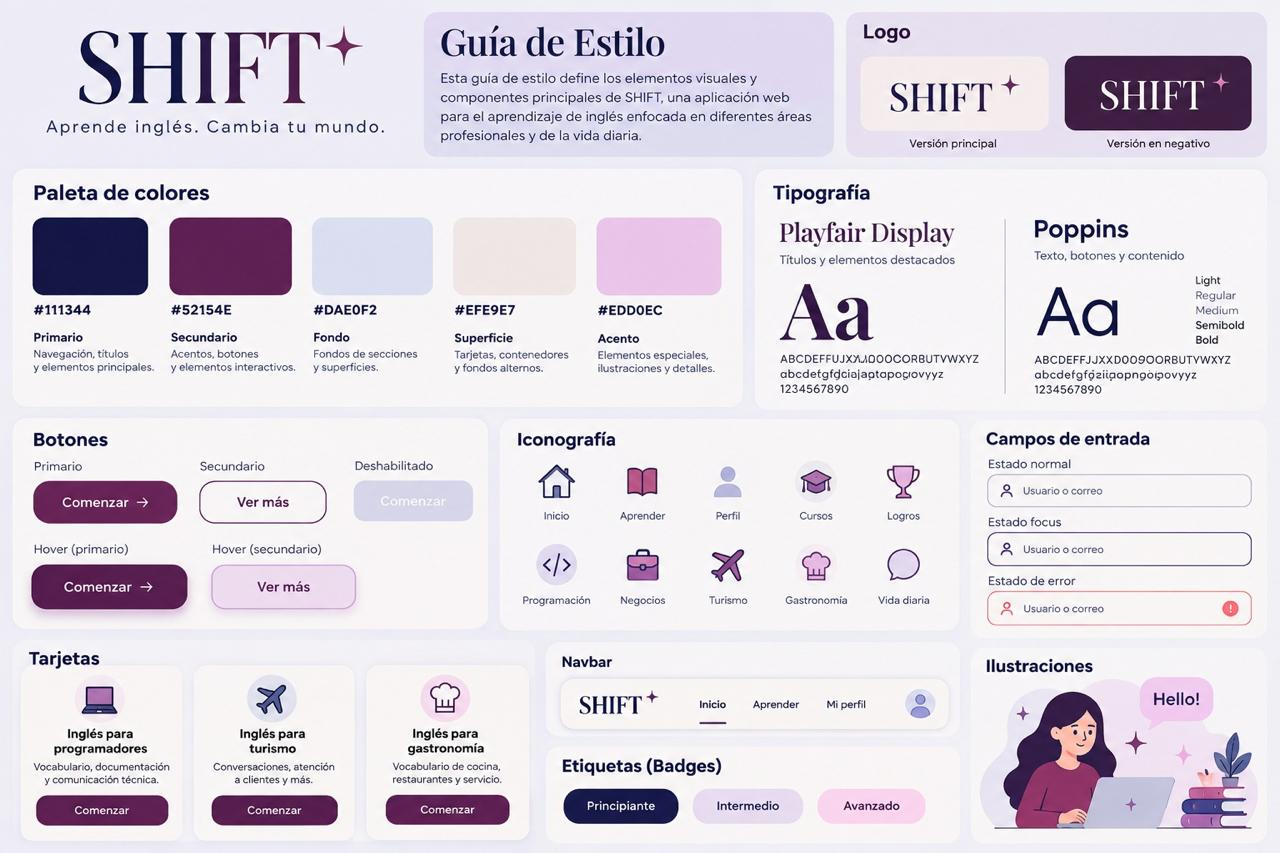
\includegraphics[width=\textwidth]{Guia de estilo.jpeg}
\caption{Guía de estilo }\label{fig:Guia de estilo}
\end{figure}